% 89-06(89쪽) — $A=90^\circ$ 인 삼각형 ABC 와 변 AB·BC 위의 두 점 D·E(원문 「오른쪽 그림」).
% 스캔 화질이 낮아 TikZ 로 다시 그림. 라벨은 원문 것만 — 다섯 점 이름, $4$, $30^\circ$, $A$ 와 $D$ 의 직각 표시,
% $\seg{BE}$ 의 같음 표시(원문 스캔에 보이는 것은 이 한 곳뿐이다). $\seg{BD}$(답)의 길이는 적지 않는다.
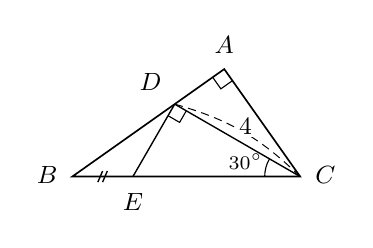
\begin{tikzpicture}[line width=0.6pt]
  \coordinate (A) at (1.930,1.365);
  \coordinate (B) at (0,0);
  \coordinate (C) at (2.894,0);
  \coordinate (D) at (1.301,0.920);
  \coordinate (E) at (0.770,0);
  \draw (A) -- (B) -- (C) -- cycle;
  \draw[line width=0.5pt] (D) -- (E);
  \draw[line width=0.5pt] (D) -- (C);
  % 직각 표시 $\angle\pt{A}$
  \draw[line width=0.4pt] (1.783,1.261) -- (1.887,1.114) -- (2.034,1.218);
  % 직각 표시 $\angle\pt{CDE}$
  \draw[line width=0.4pt] (1.448,0.835) -- (1.363,0.688) -- (1.216,0.773);
  % $30^\circ$ = $\angle\pt{DCE}$
  \draw[line width=0.4pt] (2.504,0.225) arc (150:180:0.45);
  \node[font=\scriptsize] at (2.20,0.19) {$30^\circ$};
  % $\seg{BE}$ 의 같음 표시
  \draw[line width=0.5pt] (0.325,-0.07) -- (0.385,0.07);
  \draw[line width=0.5pt] (0.385,-0.07) -- (0.445,0.07);
  % 길이 표시의 점선 호
  \draw[densely dashed, line width=0.35pt] (D) to[bend left=14] (C);
  \node[font=\small, fill=white, inner sep=1pt] at (2.20,0.64) {$4$};
  \node[font=\small, anchor=south] at (1.930,1.43) {$\pt{A}$};
  \node[font=\small, anchor=east] at (-0.06,0.02) {$\pt{B}$};
  \node[font=\small, anchor=west] at (2.96,0.02) {$\pt{C}$};
  \node[font=\small, anchor=south east] at (1.26,0.96) {$\pt{D}$};
  \node[font=\small, anchor=north] at (0.770,-0.09) {$\pt{E}$};
\end{tikzpicture}
